%%
%% This is file `sample-authordraft.tex',
%% generated with the docstrip utility.
%%
%% The original source files were:
%%
%% samples.dtx  (with options: `authordraft')
%% 
%% IMPORTANT NOTICE:
%% 
%% For the copyright see the source file.
%% 
%% Any modified versions of this file must be renamed
%% with new filenames distinct from sample-authordraft.tex.
%% 
%% For distribution of the original source see the terms
%% for copying and modification in the file samples.dtx.
%% 
%% This generated file may be distributed as long as the
%% original source files, as listed above, are part of the
%% same distribution. (The sources need not necessarily be
%% in the same archive or directory.)
%%
%% Commands for TeXCount
%TC:macro \cite [option:text,text]
%TC:macro \citep [option:text,text]
%TC:macro \citet [option:text,text]
%TC:envir table 0 1
%TC:envir table* 0 1
%TC:envir tabular [ignore] word
%TC:envir displaymath 0 word
%TC:envir math 0 word
%TC:envir comment 0 0
%%
%%
%% The first command in your LaTeX source must be the \documentclass command.
\documentclass[sigconf,authordraft]{acmart}
%% NOTE that a single column version may required for 
%% submission and peer review. This can be done by changing
%% the \doucmentclass[...]{acmart} in this template to 
%% \documentclass[manuscript,screen]{acmart}
%% 
%% To ensure 100% compatibility, please check the white list of
%% approved LaTeX packages to be used with the Master Article Template at
%% https://www.acm.org/publications/taps/whitelist-of-latex-packages 
%% before creating your document. The white list page provides 
%% information on how to submit additional LaTeX packages for 
%% review and adoption.
%% Fonts used in the template cannot be substituted; margin 
%% adjustments are not allowed.

%%
%% \BibTeX command to typeset BibTeX logo in the docs
\AtBeginDocument{%
  \providecommand\BibTeX{{%
    \normalfont B\kern-0.5em{\scshape i\kern-0.25em b}\kern-0.8em\TeX}}}

%% Rights management information.  This information is sent to you
%% when you complete the rights form.  These commands have SAMPLE
%% values in them; it is your responsibility as an author to replace
%% the commands and values with those provided to you when you
%% complete the rights form.
\setcopyright{acmcopyright}
\copyrightyear{2018}
\acmYear{2018}
\acmDOI{XXXXXXX.XXXXXXX}

%% These commands are for a PROCEEDINGS abstract or paper.
\acmConference[The Web Conference '23]{Make sure to enter the correct
  conference title from your rights confirmation email}{April 30 - May 4,
  2023}{Austin, TX}
%%
%% Submission ID.
%% Use this when submitting an article to a sponsored event. You'll
%% receive a unique submission ID from the organizers
%% of the event, and this ID should be used as the parameter to this command.
%%\acmSubmissionID{123-A56-BU3}

%%
%% For managing citations, it is recommended to use bibliography
%% files in BibTeX format.
%%
%% You can then either use BibTeX with the ACM-Reference-Format style,
%% or BibLaTeX with the acmnumeric or acmauthoryear sytles, that include
%% support for advanced citation of software artefact from the
%% biblatex-software package, also separately available on CTAN.
%%
%% Look at the sample-*-biblatex.tex files for templates showcasing
%% the biblatex styles.
%%

%%
%% For managing citations, it is recommended to use bibliography
%% files in BibTeX format.
%%
%% You can then either use BibTeX with the ACM-Reference-Format style,
%% or BibLaTeX with the acmnumeric or acmauthoryear sytles, that include
%% support for advanced citation of software artefact from the
%% biblatex-software package, also separately available on CTAN.
%%
%% Look at the sample-*-biblatex.tex files for templates showcasing
%% the biblatex styles.
%%

%%
%% The majority of ACM publications use numbered citations and
%% references.  The command \citestyle{authoryear} switches to the
%% "author year" style.
%%
%% If you are preparing content for an event
%% sponsored by ACM SIGGRAPH, you must use the "author year" style of
%% citations and references.
%% Uncommenting
%% the next command will enable that style.
%%\citestyle{acmauthoryear}

%%
%% end of the preamble, start of the body of the document source.
\begin{document}

\def\yy#1{{\color{red}\textbf{yy: #1}}\xspace}
\def\sk#1{{\color{blue}\textbf{SK: #1}}\xspace}
%%
%% The "title" command has an optional parameter,
%% allowing the author to define a "short title" to be used in page headers.
\title{Fairness through Biased Sampling: Learning to distinguish Good from Evil}


%%
%% The "author" command and its associated commands are used to define
%% the authors and their affiliations.
%% Of note is the shared affiliation of the first two authors, and the
%% "authornote" and "authornotemark" commands
%% used to denote shared contribution to the research.
% \author{Ashutosh Tiwari}
% % \authornote{Both authors contributed equally to this research.}
% \affiliation{%
%   \institution{Center for Complex Networks and Systems Research, Indiana University}
%   % \streetaddress{Luddy School of Informatics, Computing and Engineering, Indiana University}
%   \city{Bloomington}
%   \state{Indiana}
%   \country{USA}
%   \postcode{47408}
% }
% \email{ashutiwa@iu.edu}
% \author{Sadamori Kojaku}
% \affiliation{%
%   \institution{Center for Complex Networks and Systems Research, Indiana University}
%   % \streetaddress{Luddy School of Informatics, Computing and Engineering, Indiana University}
%   \city{Bloomington}
%   \state{Indiana}
%   \country{USA}
%   \postcode{47408}
% }
% \email{skojaku@iu.edu}
%
% \author{Yong-Yeol Ahn}
% \affiliation{%
%   \institution{Center for Complex Networks and Systems Research, Indiana University}
%   % \streetaddress{Luddy School of Informatics, Computing and Engineering, Indiana University}
%   \city{Bloomington}
%   \state{Indiana}
%   \country{USA}
%   \postcode{47408}
% }
% \email{yyahn@iu.edu}


%%
%% By default, the full list of authors will be used in the page
%% headers. Often, this list is too long, and will overlap
%% other information printed in the page headers. This command allows
%% the author to define a more concise list
%% of authors' names for this purpose.
% \renewcommand{\shortauthors}{Trovato and Tobin, et al.}

%%
%% The abstract is a short summary of the work to be presented in the
%% article.
\begin{abstract}
Graph data is pervasive in technology and social domain such as social networks and the Internet. The increasing use of graph data has led to an increased emphasis on the fairness of its applications. For instance, many social networks exhibit strong homophily for gender, race, and ethnicity, which AI systems may use to make critical decisions such as promotions and hiring. Previous approaches focus on manipulating input data or the output embedding. However, manipulation can cause representational harm because it may substantially degenerate the quality of embedding and introduce new biases. Here, we provide a simple, non-parametric and versatile training framework to jointly optimize the quality and fairness of embedding. Our training framework leverages an organic debiasing capacity of contrastive learning which trains a model by discriminating between positive and negative examples. We bias the sampling of negative examples such that biases are not informative in the discrimination, preventing the model from using bias for the discrimination task. Our framework can be applied to a wide spectrum from simple neural networks to more complex and deeper graph neural networks. Using link prediction as an application, we demonstrate that our approach substantially reduces multiple biases while keeping high accuracy.
\end{abstract}

%%
%% The code below is generated by the tool at http://dl.acm.org/ccs.cfm.
%% Please copy and paste the code instead of the example below.
%%

\begin{CCSXML}
<ccs2012>
   <concept>
       <concept_id>10010147.10010257</concept_id>
       <concept_desc>Computing methodologies~Machine learning</concept_desc>
       <concept_significance>500</concept_significance>
       </concept>
   <concept>
       <concept_id>10003752.10010070</concept_id>
       <concept_desc>Theory of computation~Theory and algorithms for application domains</concept_desc>
       <concept_significance>500</concept_significance>
       </concept>
   <concept>
       <concept_id>10010405.10010455.10010461</concept_id>
       <concept_desc>Applied computing~Sociology</concept_desc>
       <concept_significance>100</concept_significance>
       </concept>
 </ccs2012>
\end{CCSXML}

\ccsdesc[500]{Computing methodologies~Machine learning}
\ccsdesc[500]{Theory of computation~Theory and algorithms for application domains}
\ccsdesc[100]{Applied computing~Sociology}
%% Keywords. The author(s) should pick words that accurately describe
%% the work being presented. Separate the keywords with commas.
\keywords{Graph Embedding, Fairness Aware, Contrastive Learning}


%%
%% This command processes the author and affiliation and title
%% information and builds the first part of the formatted document.
\maketitle

\section{Introduction}
Bias is an inseparable part of output models of considerable size. This bias is generally the result of data itself on which model is trained. This bias is tackled at different stages in previous attempts. Some previous works' suggest that we should fix it at the level of raw data itself. However in most of cases this bias is not trivial to be identified at that level both because of the scale and in some cases inability to identify bias at a granular level by human supervision.
\section{Related Work}

\section{Method}

Our training framework is built on a debiasing feature of negative sampling~\cite{kojaku_residual2vec_2021}. In what follows, we summarizes the debiasing feature of negative sampling and introduce our notation.
Modifying the template --- including but not limited to: adjusting
margins, typeface sizes, line spacing, paragraph and list definitions,
and the use of the \verb|\vspace| command to manually adjust the
vertical spacing between elements of your work --- is not allowed.



\subsection{Set up and notation}
We assume that a graph consisting of $N$ nodes and $M$ edges. Each node $i$ has a $K$-dimensional vector $x_i$ representing the $i$'s attributes. Each edge $(i,j)$ between nodes $i$ and $j$ can be directed and have weight $w_{ij}$. We assume that the given graph is weakly connected.

Our goal is to create an embedding that has no information about a categorical sensitive attribute such as gender and ethnicity. We denote by $c_i$ the sensitive attribute of node $i$. We consider a node-centric fairness; we consider that an embedding is fair with respect to a sensitive attribute $c_i$ if the distance from each node $i$ to other nodes in each categorical group is indistinguishable. For instance, an embedding of social networks is fair with respect to gender if an individual is equally close to all gender groups.

\subsubsection{Biases in negative sampling}

Negative sampling is a simplified version of noise contrastive learning (NCE)~\cite{Gutmann2010}. This simplification leads to a remarkable debiasing feature~\cite{kojaku_residual2vec_2021}, which is at the heart of our approach. NCE is a generic method to fit probability model
\begin{align}
P(x) = \frac{1}{Z}\exp\left[f(x;\theta)\right], \label{eq:nce}
\end{align}
where $x$ is an entity with support ${\cal X}$, $f$ is a real-valued function, $\theta$ is parameters to estimate, $Z$ is a normalization constant. word2vec is a special case with $x=(i,j)$ and $f(i,j) = u_i^\top v_j$. NCE fits the probability model by discriminating a data sample $x$ sampled from a given dataset and $x'$ sampled from a random distribution $P_0$ using logistic regression model
\begin{align}
P\left(Y_{ij} = 1\right):= \frac{1}{1 + \exp(-f(x) + \ln P_0(x))},
\end{align}
where $Y_i = 1$ if pair $(i,j)$ comes from a given data, and $Y_{ij}=0$ otherwise. Notably, NCE is an asymptomatically unbiased estimator of Eq.~\ref{eq:nce}~\cite{Gutmann2010,Dyer2014}. Negative sampling simplifies the logistic function by dropping $\ln P_0(x)$, i.e.,
\begin{align}
P\left(Y_{ij} = 1\right):= \frac{1}{1 + \exp(-f(x))}, \label{eq:negative_sampling}
\end{align}
An important consequence is that this simplification yields an estimation bias. To see the bias, let us rewrite Eq.~\ref{eq:negative_sampling} in form of NCE as
\begin{align}
P\left(Y_{ij} = 1\right):= \frac{1}{1 + \exp\left[-\left(f(x) + \ln P_0(x) \right)+ \ln P_0(x)\right]}, \label{eq:negative_sampling_nce}.
\end{align}
By defining $f'(x)=f(x) + \ln P_0(x)$ and substituting it to Eq.~\ref{eq:nce}, one shows that negative sampling is unbiased estimator of the following model~\cite{kojaku_residual2vec_2021}:
\begin{align}
P(x) = \frac{1}{Z'}P_0(x)\exp\left[f(x;\theta)\right].
\end{align}
Notably, random distribution $P_0$ becomes a component in the model and manifests the estimation bias of negative sampling.

\subsubsection{Debiasing for graph representation learning}

Many graph representation is generated based on node triplets $(i,j,j')$ encoding local structure around each node $i$; node $j$ represents a context randomly sampled from the neighborhood of node $i$, where the neighborhood refers to direct neighbors neighbors~\cite{tangLINELargescaleInformation2015} or nodes with close proximity~\cite{perozziDeepWalkOnlineLearning2014,groverNode2vecScalableFeature2016}. Node $j'$ represents a \textit{random} context sampled from a random distribution $P_0(j')$.
One generates a graph embedding by discriminating actual context $j$ and random context $j'$ by using a logistic function:
\begin{align}
\frac{1}{1 + \exp(-u_i ^\top v_j)},
\end{align}
where $u_i$ and $v_i$ are the in-vector and out-vector that represent a node $i$ as an anchor and context node respectively.
This training process is negative sampling, and thus, learns probability model
\begin{align}
P(j \vert i) = \frac{1}{Z'}P_0(j)\exp\left(u_i ^\top v_j\right), \label{eq:graph_representation_model}
\end{align}
where $P(j\vert i)$ is the probability that $j$ is sampled from the neighborhood of $i$, representing a structural association between nodes $i$ and $j$. Equation~\ref{eq:graph_representation_model} decomposes the structural association into $P_0(j)$ and $\exp\left(u_i ^\top v_j\right)$, where $P_0(j)$ plays a role as a \textit{baseline} probability, and embedding vectors $u_i$ and $v_j$ encode \textit{residual} not explained by the baseline.
residual2vec utilizes this implicit decomposition for debiasing a shallow neural network---word2vec---for graph representation learning~\cite{kojaku_residual2vec_2021}.
The key idea is to explicitly model $P_0$ that accounts for the structural associations attributed to a focal bias and train embedding on the residual unbiased component.
For instance, for a social network with strong gender homophily, one can generate a gender-neutral embedding by using a biased baseline $P_0$ that samples a random context node $j'$ whose distribution is statistically indistinguishable with actual context $j$ with respect to gender. Since both contexts $j$ and $j'$ are indistinguishable by gender, embedding---which is trained to distinguish $j$ and $j'$ by negative sampling---learns something other than gender.

\subsection{(Put the name of the proposed method)}

Building on residual2vec, we propose a general training framework for more complex graph neural networks. The key idea is that negative sampling is agnostic to how embedding $u_i$ is generated and what it is generated from. Thus, we can define $u_i:=\phi_{\text{in}}(i, A, X)$ and $v_i:=\phi_{\text{out}}(j, A, X)$ with any graph neural networks $\phi_{\text{in}}$ and $\phi_{\text{out}}$ that take node features $\mat{X}$ and the adjacency matrix $\mat{A}$. The graph neural networks learn a probability model:
\begin{align}
P(j \vert i) = \frac{1}{Z'}P_0(j\vert i)\exp\left[\phi_{\text{in}}(i, A, X) ^\top \phi_{\text{out}}(j, A, X)\right]. \label{eq:proposed}
\end{align}
Let us demonstrate the effectiveness of our approach using a small toy network, namely political book network.
This network consists of ... \sk{Write a description of the political book network.}
We aim to create an embedding that is neutral with respect to the political leaning. To this end, we use a baseline $P_0(j\vert i)$ proposed in the previous study \cite{kojaku_residual2vec_2021} that accounts for structural biases pertained to a categorical variable (i.e., political learning in our toy example).
We generate triplets $(i,j,j')$, where context $j$ is sampled from direct neighbors of $i$.
We train (GNNs you like) on the generated triplets and use the $K=???$ eigenvectors of the normalized(do we? node2vec?) Laplacian matrix as the node features.

\begin{figure}[h]
  \centering
  \includegraphics[width=\linewidth]{images/demonstration/biased.png}
  \caption{Biased Embeddings (PCA)}
\end{figure}

\begin{figure}[h]
  \centering
  \includegraphics[width=\linewidth]{images/demonstration/word2vec.png}
  \caption{Word2vec }
\end{figure}

\begin{figure}[h]
  \centering
  \includegraphics[width=\linewidth]{images/demonstration/gat.png}
  \caption{GAT(PCA)}
\end{figure}

\begin{figure}[h]
  \centering
  \includegraphics[width=\linewidth]{images/demonstration/gcn.png}
  \caption{GCN(PCA)}
\end{figure}
Figure~\ref{fig:political_book} shows the original and debiased embedding. \sk{write the results}

\section{Experiments}
We used there 4 networks for our analysis ~\ref{table:datasets}. There size and other particulars are included in next section. For each of these datasets we trained 5 pairs of GNN models ~\ref{table:models} each with combination crosswalk and ~\sk{name of method}.

All of these experiments are repeated 5 times and are reported in results. Each time the network is divided into a test and train network. Test edges are selected from non MST edges which are a fraction of $.5$ of total edges and the train edges forming the rest of the network.

All of these models take $16$ dimensional node2vec ~\cite{grover_node2vec_2016} node features as the input for every corresponding triplet node (center, positive and random). These Node2Vec models are trained differently in case when crosswalk is involved or not. In case when crosswalk is used node2vec is trained on "weighed" adjacency matrix compared to a binary one in case it is not used.

\subsection{Models}
\sk{AT add number of layers etc and overall architecture of ivs and ovs for each dataset}

This method is independent of the model used to encode network nodes. In this case we show word2vec, GAT and GCN. We also show the results of the baseline method which is the same as the proposed method but the negative samples are generated randomly from the network. Here is the structure of GAT and GCN, models used in this paper.

The input to our model 

% \begin{table*}[h]
%   \caption{Models}
%   \label{table:models}
%   \begin{tabular}{ccl}
%     \toprule
%     NAME  & DESCRIPTION\\
%     \midrule
%     GCN & 5 Layers of GCNConv (~\cite{kipf2017semisupervised}) followed by a dropout of .2 \\
% GAT & 5 layers of GATConv(~\cite{https://doi.org/10.48550/arxiv.1710.10903}) followed by a dropout of .2\\
%     \bottomrule
%   \end{tabular}
% \end{table*}

\subsection{Datasets}
\sk{AT add dataset cites here}
We use 4 datasets in this work. There is small pokec dataset which is created from set of nodes in pokec dataset where degree is more than $45$. All of these networks are treated as undirected networks.

\begin{table}[h]
  \caption{Datasets}
  \label{table:datasets}
  \begin{tabular}{ccl}
    \toprule
    NAME & \#  NODES & \# EDGES\\
    \midrule
    Pokec       & $1632803$ & $22301964$ \\
    Small Pokec & $406898$ & $11627007$  \\
Airport & $2898$ & $15564$  \\
Polbook         &$105$&$441$  \\
Polblog         & $1224$ & $16715$  \\\
    \bottomrule
  \end{tabular}
\end{table}

\subsection{Link prediction benchmark}
\sk{AT: How these ROC scores were obtained.}

To calculate these ROC AUC scores we take a test network and then sample negative edges. We then generate ivectors for each of the nodes and then use their dot product as the as the predicted value and whether they are connected or not as the target.
\begin{figure}[h]
  \centering
  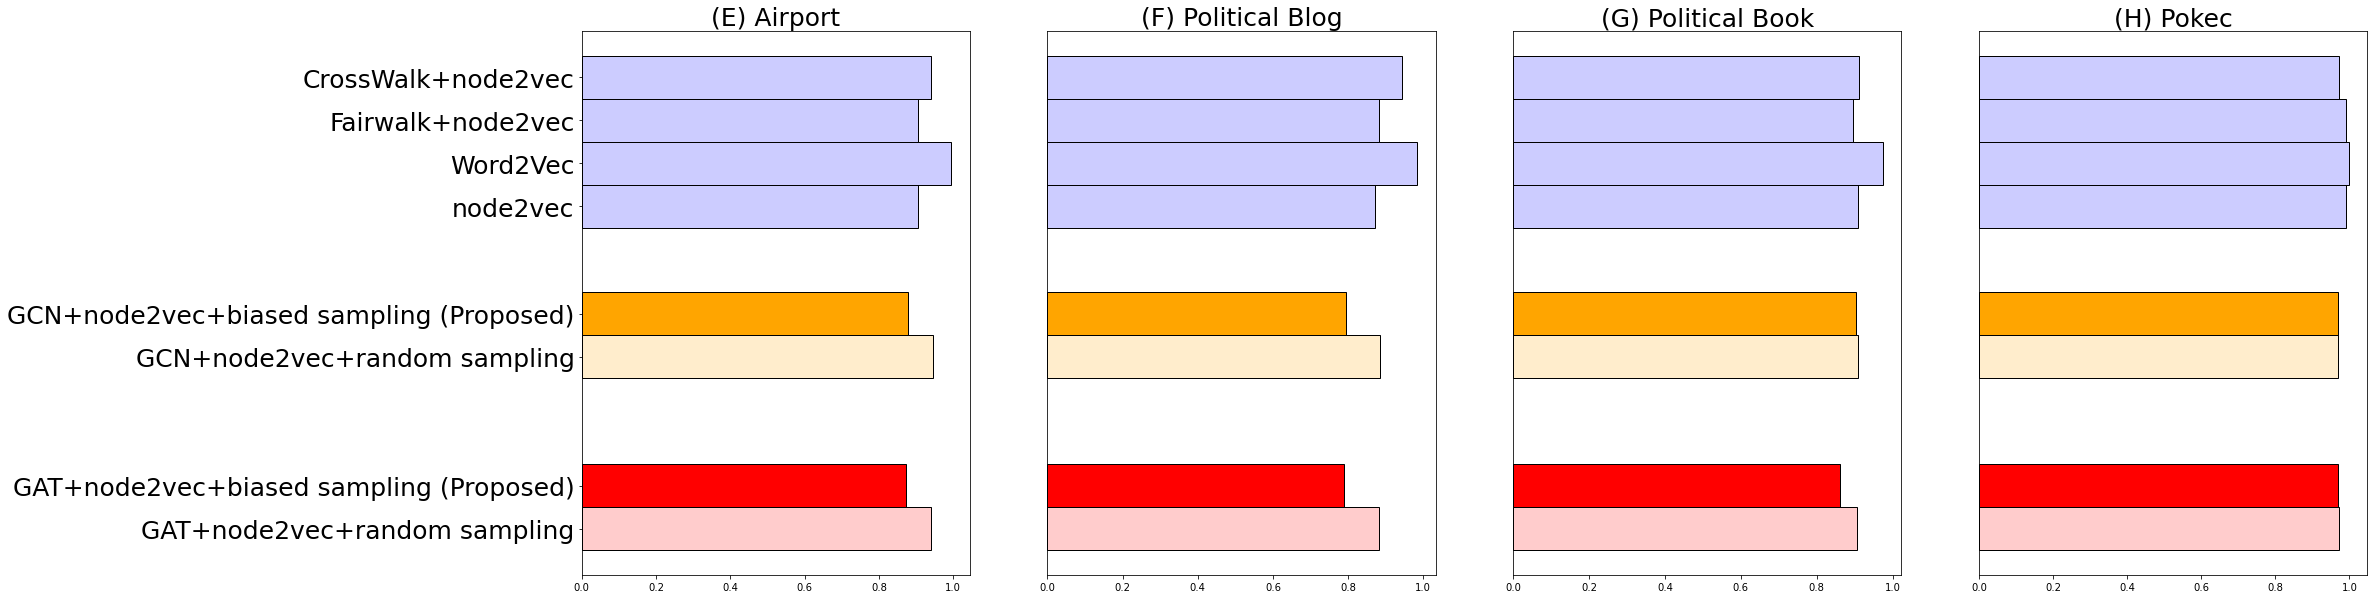
\includegraphics[width=\linewidth]{images/bar_roc.png}
  \caption{ROC AUC scores}
  \Description{Mean ROC AUC Scores across runs}
\end{figure}
\begin{figure}[h]
  \centering
  \includegraphics[width=\linewidth]{images/bar_gini.png}
  \caption{gini scores}
  \Description{Mean gini scores across runs}
\end{figure}
\begin{figure}[h]
  \centering
  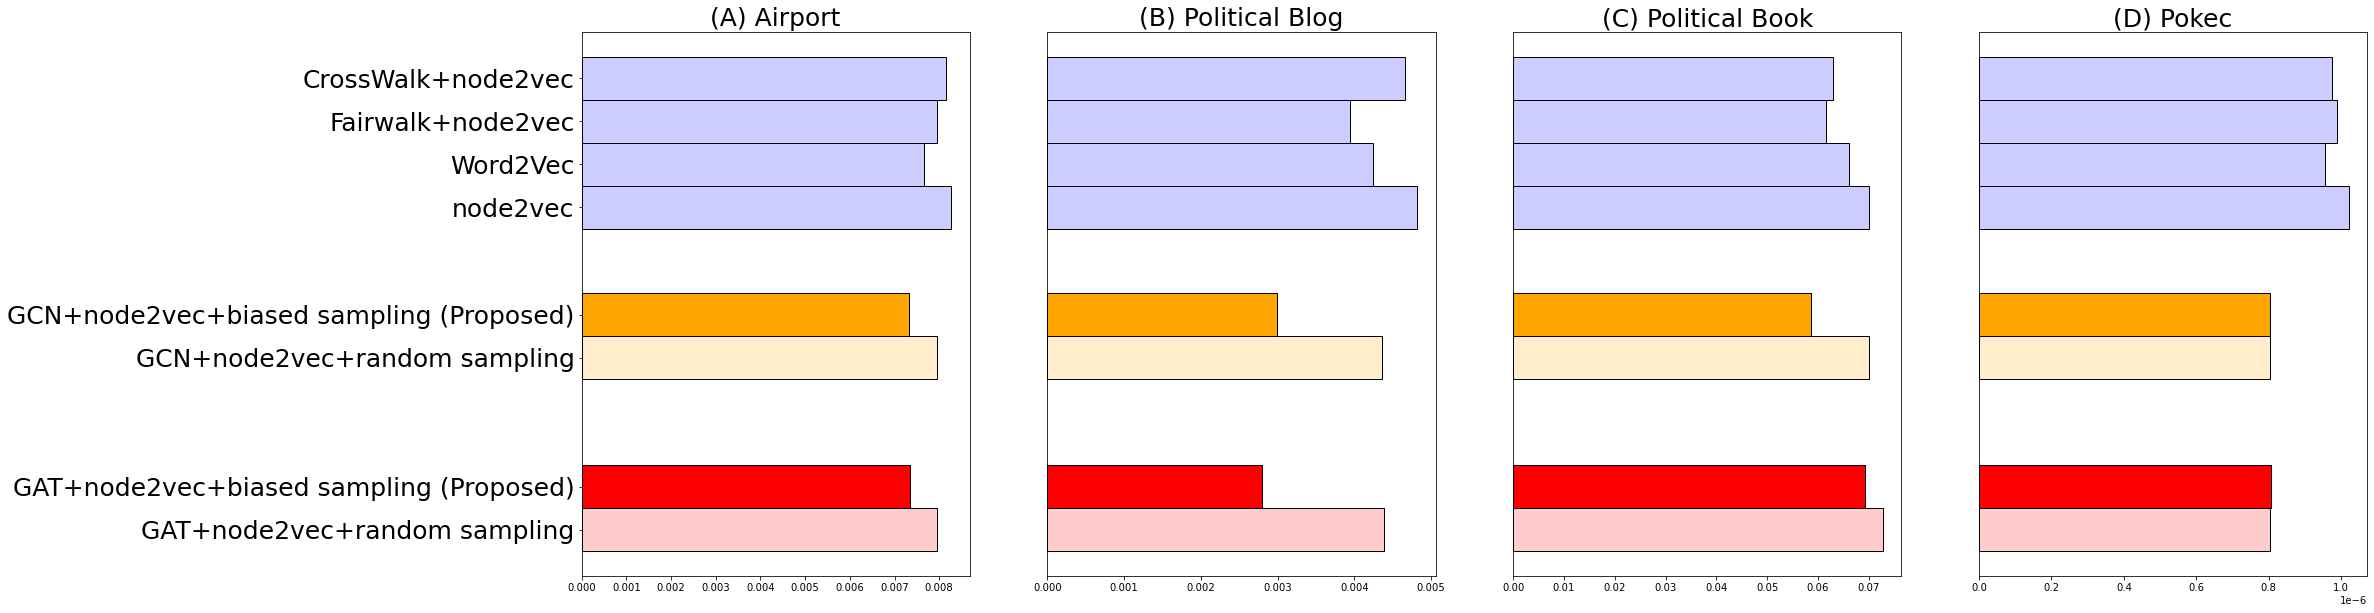
\includegraphics[width=\linewidth]{images/bar_sp.png}
  \caption{Statistical Parity scores}
  \Description{Mean Statistical Parity Scores across runs}
\end{figure}

\begin{figure}[H]

  \centering
  \includegraphics[width=\linewidth]{images/swarm_airport.png}
  \caption{Airport Dataset Scores}
  \Description{Scores for each run}
\end{figure}
\begin{figure}[H]

  \centering
  \includegraphics[width=\linewidth]{images/swarm_polbook.png}
  \caption{Polbook Dataset Scores}
  \Description{Scores for each run}
\end{figure}

\begin{figure}[H]

  \centering
  \includegraphics[width=\linewidth]{images/swarm_polblog.png}
  \caption{Polblog Dataset Scores}
  \Description{Scores for each run}
\end{figure}

\begin{figure}[H]
  \centering
  \includegraphics[width=\linewidth]{images/swarm_small_pokec.png}
  \caption{Small Pokec Dataset Scores}
  \Description{Scores for each run}
\end{figure}
\begin{figure}[H]
  \centering
  \includegraphics[width=\linewidth]{images/swarm_pokec.png}
  \caption{Pokec Dataset Scores}
  \Description{Scores for each run}
\end{figure}

\begin{figure}[H]

  \centering
  \includegraphics[width=\linewidth]{images/box_airport.png}
  \caption{Airport Dataset Scores}
  \Description{Scores for each run}
\end{figure}

\begin{figure}[H]

  \centering
  \includegraphics[width=\linewidth]{images/box_polbook.png}
  \caption{Polbook Dataset Scores}
  \Description{Scores for each run}
\end{figure}
\begin{figure}[H]

  \centering
  \includegraphics[width=\linewidth]{images/box_polblog.png}
  \caption{Polblog Dataset Scores}
  \Description{Scores for each run}
\end{figure}

\begin{figure}[H]

  \centering
  \includegraphics[width=\linewidth]{images/box_small_pokec.png}
  \caption{Small Pokec Dataset Scores}
  \Description{Scores for each run}
\end{figure}
\begin{figure}[H]

  \centering
  \includegraphics[width=\linewidth]{images/box_pokec.png}
  \caption{Pokec Dataset Scores}
  \Description{Scores for each run}
\end{figure}
\begin{figure}[H]

  \centering
  \includegraphics[width=\linewidth]{images/roc_sp.png}
  \caption{ROC AUC vs Statistical Parity}

\end{figure}
\begin{figure}[H]

  \centering
  \includegraphics[width=\linewidth]{images/roc_gini.png}
  \caption{ROC AUC vs Gini SP Scores}

\end{figure}
\section{Conclusion}



%%
%% The acknowledgments section is defined using the "acks" environment
%% (and NOT an unnumbered section). This ensures the proper
%% identification of the section in the article metadata, and the
%% consistent spelling of the heading.
\begin{acks}
% To Robert, for the bagels and explaining CMYK and color spaces.
\end{acks}

%%
%% The next two lines define the bibliography style to be used, and
%% the bibliography file.
\bibliographystyle{ACM-Reference-Format}
\bibliography{sample-base}

%%
%% If your work has an appendix, this is the place to put it.
\appendix


\end{document}
\endinput
%%
%% End of file `sample-authordraft.tex'.
